\documentclass[10pt,letterpaper]{article}
% RECOMB 2027: max 10 Letter pages incl. figures/tables and captions; >= 10 pt; 1-inch margins;
% an extra title page (title, authors, abstract) is allowed; the bibliography does not count.
% The appendix is a separate supplementary PDF (supplement.tex); reviewing it is optional.
\usepackage[letterpaper,margin=1in]{geometry}
\usepackage[T1]{fontenc}
\usepackage{mathptmx}
\usepackage{graphicx,booktabs,amsmath,amssymb,amsthm,tabularx,xcolor,microtype}
\usepackage[font=normalsize,labelfont=bf,skip=4pt]{caption}
\usepackage[numbers,sort&compress]{natbib}
\usepackage[hidelinks]{hyperref}
\usepackage{enumitem}
\usepackage{placeins}
\setlist{nosep,leftmargin=1.4em}
\graphicspath{{../figures/}}
\newcommand{\coderepo}{\url{https://github.com/Tears-0/smalln-bench}}
\newtheorem{proposition}{Proposition}
\usepackage{etoolbox}
\patchcmd{\abstract}{\small}{\normalsize}{}{}   % abstract heading and text at 10 pt (RECOMB minimum)
\usepackage{authblk}
\renewcommand\Authfont{\normalsize}
\renewcommand\Affilfont{\normalsize}
\renewcommand{\floatpagefraction}{0.85}
\renewcommand{\topfraction}{0.9}

\title{When can a small proteomics study trust its cross-validated AUC?\\
A null-calibration condition and a pre-specified benchmark}
\author[1]{Chong Chi Yang}
\author[1]{Ong Huey Fang}
\author[2]{Michelle Yap Khai Khun}
\affil[1]{School of Information Technology, Monash University Malaysia, Bandar Sunway, Malaysia}
\affil[2]{School of Science, Monash University Malaysia, Bandar Sunway, Malaysia}
\affil[ ]{\texttt{chiyang80@gmail.com}, \texttt{ong.hueyfang@monash.edu}, \texttt{Yap.Michelle@monash.edu}}
\date{}

\begin{document}
\maketitle
\thispagestyle{empty}

\begin{abstract}
\normalsize\noindent
Wet-lab proteomics studies often have fewer than a dozen samples, and their only evidence that a classifier
generalises is the study's own cross-validated AUC. We give a condition under which such an internal
estimate is calibrated, and test it at scale. When labels carry no information, any estimator whose every
comparison is between two held-out samples scored by one model trained without either---leave-pair-out, or
$k$-fold with AUC computed per fold---has expected AUC exactly 0.5, whatever the learner and in-fold pipeline. Pooled leave-one-out
(LOOCV) AUC breaks the condition: it compares scores from models whose training class balance depends on
the held-out label, so its bias takes a sign set by the learner. The condition also yields a
permutation-null leakage test; on its 25 checks, the pre-specified decision rule would flag a clean pipeline
with probability 0.91, and a one-sided rule on the mean lowers this to 0.07. We then subsampled
three public mass-spectrometry cohorts (CPTAC lung tumour versus normal tissue; TP53 status in CPTAC
pancreatic tumours and in ProCan-DepMapSanger haematopoietic cell lines) to $N = 6$--$50$, 100 times each,
with patient-disjoint held-out sets, and ran 15 configurations (compound covariate predictor, elastic net,
random forest, TabPFN, a protein-language-model fusion network, and pipeline variants) under true and
permuted labels: 51,000 runs. The design was fixed before the first run, and every later change is reported. As the
condition predicts, pooled LOOCV erred by $-0.60$ to $+0.29$ depending on the learner, with errors of the
same sign and similar size under permuted labels; the positive extreme came from the fusion network, which
assigns held-out samples to the training minority class. Leave-pair-out stayed within $\pm 0.08$ for all
five models. From $N = 20$, $k$-fold was right on average but overstated held-out AUC by more than 0.1 in
17--23\% of studies at $N = 20$--$30$. Selecting features before cross-validation inflated the estimate by
up to 0.45, and from $N = 20$ SMOTE before the split added 0.07--0.16 more. In the two weak-signal tasks, top-50 protein
lists from different subsamples overlapped little more than chance, no model was reliably best, and no
pipeline variant helped. In follow-up runs, each fixed in a written plan before fresh draws, protein-language-model
and co-expression embeddings added nothing, whereas a TP53 signature fitted to other cohorts and applied
without the study's labels beat all four standard models trained on the study's own samples at $N = 12$ and 30.
\end{abstract}

\noindent\textbf{Code and data:} \coderepo{} (all benchmark datasets are public; supplementary material in a
separate PDF).
\newpage
\setcounter{page}{1}

% =====================================================================================
\section{Introduction}

Proteomic biomarker studies in cell models and small clinical series routinely work with nine, twelve or
twenty samples against thousands of proteins. Such a study cannot hold out an independent test set: its
evidence that a classifier generalises, and that its top-ranked proteins are worth following up, comes from
cross-validation (CV) on the same handful of samples. Two failure modes of CV at small $N$ are known from
microarray studies: supervised feature selection before CV leaks the test labels into the model
\citep{ambroise2002selection,varma2006bias}, and leave-one-out CV (LOOCV) on balanced classes
anti-correlates training and held-out labels \citep{parker2007stratification}, which makes pooled
leave-one-out AUC unreliable \citep{airola2011auc}. Missing is a statement of when an internal AUC estimate
is calibrated at all, and a measurement, on real mass-spectrometry data, of how far it departs from
held-out performance at a laboratory's own $N$.

We address both. First, we state a symmetry condition (Proposition~\ref{prop:null}): if every comparison an
AUC estimator makes is between two samples scored by the same model, trained without either, with weights and
folds that treat the two labels alike, its expected value under uninformative labels is exactly 0.5 for any
learner. Leave-pair-out and per-fold $k$-fold meet
the condition; pooled LOOCV does not, and its bias can then be negative or positive, depending on how the
learner responds to the class balance of its training set. The condition gives leakage testing a known
null, and we calibrate such a test for small-$N$ discreteness. Second, we measure internal estimates on
large public cohorts treated as populations: we draw small balanced subsamples, score every method by its
own internal CV and on the samples it never saw, and take the difference---the optimism a small study
cannot compute for itself. We also ask whether top-ranked proteins match the full cohort's, and whether
selection stability, which a small study \emph{can} compute, predicts that.

The work was motivated by a study from our collaborating laboratory: label-free LC--MS/MS of HaCaT
keratinocytes, untreated or exposed to a snake-venom cytotoxin for 8 or 24 hours, three biological
replicates per condition---nine samples in three classes, 2,841 quantified protein accessions, 54.3\% of
values missing. An earlier, unpublished analysis of these data proposed a fusion network combining protein
abundance with embeddings from the protein language model ESM-2 \citep{lin2023esm2}, and could estimate its
performance only by resampling the same nine samples. The study has no held-out samples, so it supplies no
evidence here; its architecture is one benchmark arm, and \S\ref{sec:case} illustrates both internal
estimators on its data. We make no biological claims.

\paragraph{Contributions.}
\begin{enumerate}
  \item A null-calibration condition for internal AUC estimators (Proposition~\ref{prop:null}), which
        explains the learner-dependent sign of pooled-LOOCV bias and is borne out by the 25,500
        permuted-label runs, including a learner whose pooled-LOOCV bias is positive.
  \item A permutation-null leakage test built on the condition, with its decision rule calibrated for
        small-$N$ discreteness (false-alarm probability 0.91 for the pre-specified rule, 0.07 for the
        amended one).
  \item A pre-specified subsampling benchmark on three public cohorts, two acquisition platforms (TMT,
        DIA), one large-effect and two weak-signal tasks, with patient-disjoint draws, measuring optimism
        from $N = 6$ to $50$ and the cost of two leaky practices.
  \item A decision table for small laboratories that also states the claims the evidence does not support,
        and a record of every deviation from the pre-specified design.
\end{enumerate}

\paragraph{Related work.} Each failure mode we measure has been described before. Pooling scores across
folds biases AUC, most strongly under LOOCV \citep{parker2007stratification,forman2010apples,airola2011auc},
and leave-pair-out was found nearly unbiased in simulation \citep{airola2011auc}; Proposition~\ref{prop:null}
states the exact null property and the condition behind it. Oversampling before the split inflates
cross-validated performance \citep{santos2018cross}, and at small $N$ CV estimates carry error bars as wide as
the effects they report \citep{varoquaux2018cross,vabalas2019machine}. In microarray studies, gene lists from
different training sets barely overlapped \citep{eindor2006thousands,michiels2005prediction}, predictor
accuracy was mapped against training-set size and task difficulty \citep{popovici2010effect}, and MAQC-II
compared validation practice across many teams on independent data \citep{shi2010maqc}. In proteomics, the
scarcity of validated biomarkers has been traced to small discovery cohorts without independent validation
\citep{hernandez2014proteomics}. The nearest study \citep{lee2024small} compared nine analysis schemes on
simulated SOMAScan data (1,317 proteins, 26 subjects), estimating performance by LOOCV with bootstrap
optimism correction and no external test set, and found near-perfect internal performance that signalled
overfitting, with heterogeneous selected protein sets. We add the null condition, a calibrated leakage test,
and a measurement of these effects side by side on real mass-spectrometry cohorts with their own
missingness, from $N = 6$, against held-out samples, for current models including a tabular foundation
model \citep{hollmann2025tabpfn,tabpfn2026v35} and a protein-language-model fusion network.

% =====================================================================================
\section{Null calibration of internal AUC estimates}\label{sec:theory}

\subsection{A symmetry condition}
Let a study hold $N$ samples with features $x_1, \dots, x_N$ and labels $y \in \{0, 1\}^N$, $n_1$ of them
positive. A \emph{pipeline} maps a labelled training set to a scoring function $f$; it includes every
preprocessing step fitted on that set and may be randomised, with randomness independent of $y$. Comparing
a positive $i$ with a negative $j$ by $f$ scores $c(f; i, j) = \mathbb{1}[f(x_i) > f(x_j)] +
\tfrac12 \mathbb{1}[f(x_i) = f(x_j)]$, so that $c(f; i, j) + c(f; j, i) = 1$. An internal AUC estimator draws
a fold plan, fits one model per fold, and averages comparisons between test samples. We call it
\emph{pair-symmetric} if (a)~each comparison of $i$ and $j$ uses a single model whose training set contains
neither; (b)~the weight of each comparison depends only on class counts; and (c)~exchanging the labels of
two samples changes neither whether they are compared nor the distribution of the fit that compares them. Leave-pair-out, which
fits one model per positive--negative pair on the other $N - 2$ samples, meets (a)--(c); so does $k$-fold
with AUC computed within each fold and averaged, when folds are drawn uniformly within each class, as
stratified splitting does. Under the \emph{null}, $y$ is independent of the features given the class
counts, i.e.\ uniform over the $\binom{N}{n_1}$ labellings---exactly the permuted-label arm of our benchmark.

\begin{proposition}\label{prop:null}
Under the null, every pair-symmetric estimator has expected value $1/2$ given $x_1, \dots, x_N$, for any
pipeline.
\end{proposition}

\begin{proof}
The estimate is a sum of terms $w \, c(f; \text{positive}, \text{negative})$ over the fits and the
oppositely labelled pairs $\{i, j\}$ compared in them, with weights summing to 1. Fix a pair and condition on
the labels of all other samples. Under the null the two ways of labelling $i$ and $j$ oppositely are equally
likely. Their labels never enter the fit that compares them (a); whether they are compared, and the
distribution of that fit, are the same under both labellings (c), and so is the weight (b). The pair's expected contribution is therefore
$\tfrac12 w \, \mathbb{E}[c(f; i, j) + c(f; j, i)] = w/2$, and summing over pairs gives $1/2$.
\end{proof}

Pooled LOOCV breaks (a): it compares $f_{-i}(x_i)$ with $f_{-j}(x_j)$, scores from two models, and the
training set of $f_{-i}$ holds one fewer sample of $i$'s class. Its null expectation is $\tfrac12$ plus a
bias whose sign depends on how a held-out score responds to that class balance. At even $N$, and at $N = 9$
(classes 5/4) when the held-out sample comes from the smaller class, the held-out class is the minority of
its training fold. A learner that leans towards the training majority, through an intercept or prior, then
scores the held-out sample against its own label, and the bias is negative
\citep{parker2007stratification,airola2011auc}. A learner that pushes unusual samples towards the minority
class does the opposite: a held-out sample did not contribute to the training mean and variance, looks
unusual on the selected features, and the bias is positive. \S\ref{sec:optimism} finds both. The
proposition also says what leave-pair-out does not need: its training classes are unbalanced at odd $N$
(removing a pair from 5/4 leaves 4/3); it works because both members of each pair are scored by one model.

\subsection{A calibrated leakage test}\label{sec:leaktest}
Proposition~\ref{prop:null} gives leakage testing a known null. A leak---any route by which information from
the test samples reaches the fitted model---breaks (a), so the proposition no longer fixes the mean; a leak
that carries label information raises it above 0.5 on permuted labels. We therefore run the full pipeline on permuted labels with a pair-symmetric estimator
(leave-pair-out at $N \le 12$, per-fold $k$-fold above), and add a positive control: a deliberately leaky arm
must exceed the in-fold arm on the same draw in at least 90\% of repeats. The decision rule has to allow for
the discreteness of small-$N$ AUC. Our pre-specified rule flagged a configuration whose median internal AUC over
100 permuted-label repeats left $0.5 \pm 0.05$, across 25 configuration--$N$ checks. Leave-pair-out at
$N = 12$ moves in steps of $1/36$ with a standard deviation near 0.22, so medians wander. On the test's own
data (\S\ref{sec:gate}), with each check shifted to a mean of exactly 0.5 and whole draws resampled jointly
across configurations, which keeps their correlation, the pre-specified rule raised at least one false alarm
with probability 0.91. Label leaks raise the AUC, so a one-sided rule on the mean, alarm above 0.55, keeps the
pre-specified tolerance in the only direction that matters; its false-alarm probability is 0.07. A laboratory
can run the same test on its own pipeline, within the limits of its own labellings (Table~\ref{tab:decision}).

% =====================================================================================
\section{Benchmark design}

\subsection{Pre-specified design}
Following the logic of pre-registration \citep{nosek2018prereg}, the research question, tasks,
configurations, metrics, leakage tests and decision rules were fixed before the first benchmark run. The
design was not lodged with a public registry, so its timing rests on our own record; the code, leakage tests
and complete results are public. Every later change to the design or analysis is reported here. Before
any run, one task was
dropped because it could not meet the pre-specified rules (\S\ref{sec:tasks}); a perturbation task and a
protein-interaction smoothing arm were dropped under the pre-specified deadline rule; an external replication
track and a TabPFN pathway arm were cut for time; and the TabPFN checkpoint, which the design had left open, was
fixed. After the leakage tests but before any true-label benchmark result (a two-draw smoke test of the fusion
runner aside), the two mis-calibrated leakage tests (1 and 1b) were replaced (\S\ref{sec:gate}). After the results were known, we added the secondary analysis over B2
and B5, because the pre-specified rule could yield no claim while B1 sat at ceiling (\S\ref{sec:results});
Proposition~\ref{prop:null}; leave-pair-out for the fusion network, which the pre-specified design omitted for
cost; the other analyses marked \emph{post hoc}; the illustration on the motivating study
(\S\ref{sec:case}); and five follow-up runs, each fixed in a written plan before fresh draws, which we decided to report only after
the last (\S\ref{sec:posthoc}).

\subsection{Tasks}\label{sec:tasks}
A task is one cohort, one binary contrast and one draw unit (Table~\ref{tab:tasks}). Tasks were chosen by
pre-specified rules from sample counts and full-data effect sizes only, never from model output: never pool
cohorts or tissues (pooling makes tissue a proxy for the label); draw patients, not samples (CPTAC holds
tumour and normal tissue from the same patients); and run an $N$ only if every class keeps at least 20
samples in the held-out remainder. B1 is the CPTAC cohort with the largest min(\#tumour, \#normal adjacent
tissue (NAT)) over distinct patients \citep{gillette2020luad,lindgren2021cptac}: LUAD and LSCC tie at 102, and
the pre-specified tie-break, more samples, picks LUAD (213 vs 212). B2 is the contrast, among TP53 mutant
versus wild-type and stage I versus III--IV within each CPTAC cohort, eligible up to at least $N = 30$ with the
smallest full-data effect size \citep{cao2021pdac}; its TP53 status comes from CPTAC's \texttt{washu}
somatic-mutation calls (non-silent mutations). B5 applies the same rule to KRAS and TP53 within each tissue of
the ProCan-DepMapSanger cell lines \citep{goncalves2022procan}, with driver-mutation calls and donor
identifiers from Cell Model Passports \citep{vandermeer2019cmp}. Effect size is the median $|d|$ (Cohen's $d$)
over the full cohort's top 100 proteins. The selection, made before any model was fitted, picks the same tasks when recomputed with the statistic of Table 1 (Supplementary Table S1). We found afterwards (\emph{post hoc}) that this
statistic separates B1 from noise but not B2 or B5: with labels permuted it is 0.49 in B1, but 0.69 in B2
and 0.99 in B5, close to or above their true values of 0.77 and 0.71. B2 and B5 are therefore weak-signal
tasks, better described by their 0 and 148 FDR-significant proteins and by the held-out AUC models reach in
them (0.63--0.78 at the largest $N$ for the four baselines, 0.54--0.59 for the fusion network). Inside a
small study the statistic says even less: at $N = 6$ it is 3.7 in B2 under both true and permuted labels,
while B1 gives 7.4 against 3.5. A fourth task (ProCan tumour tissue) was dropped because its matrix carries
no patient identifiers, so patient-disjoint draws were impossible.

\begin{table}[t]
\centering
\caption{Benchmark tasks. $q<0.05$: proteins significant in the full cohort (limma, BH). Missing: fraction
of missing values in the full matrix. Median $|d|$: over the full cohort's top 100 proteins; in brackets,
the median over 20 label permutations (post hoc).}
\label{tab:tasks}
\begin{tabularx}{\textwidth}{@{}l X r r r r r l@{}}
\toprule
Task & Cohort, contrast (positive / negative) & Samples & Proteins & Missing & Median $|d|$ & $q<0.05$ & $N$ run \\
\midrule
B1 & CPTAC LUAD (TMT), tumour 111 / NAT 102; 111 patients & 213 & 13,302 & 18.9\% & 4.16 (0.49) & 10,114 & 6--50 \\
B2 & CPTAC PDAC (TMT) tumours, TP53 mutant 105 / wild-type 35 & 140 & 12,017 & 23.5\% & 0.77 (0.69) & 0 & 6--30 \\
B5 & ProCan-DepMapSanger (DIA), haem.\ lines, TP53 mutant 99 / wild-type 64 & 163 & 8,498 & 39.6\% & 0.71 (0.99) & 148 & 6--50 \\
\bottomrule
\end{tabularx}
\end{table}

\subsection{Subsampling protocol}
For each task, each eligible $N \in \{6, 9, 12, 20, 30, 50\}$ and each repeat $r = 1, \dots, 100$, a balanced
subsample $S_r$ of $N$ units---patients in B1 and B2, cell lines from 163 distinct donors in B5, so every task is
patient-disjoint---was drawn with a seed fixed by
$(\text{task}, N, r)$, so every configuration saw identical draws and all comparisons are paired. For $N = 9$
the classes were 5/4, with the larger class alternating between repeats. The held-out set $H_r$ contains
every sample from a unit not in $S_r$ (110--118 samples at the largest $N$). In B1, where most patients gave
both a tumour and a NAT sample, $S_r$ holds $N$ distinct patients and one sample from each---the tumour for a
positive, the NAT for a negative---and both samples of every patient in $S_r$ are excluded from $H_r$; in B2
and B5 each unit contributes one sample. Each draw was analysed twice: with its true labels, and with labels
permuted within $S_r$ while $H_r$ kept its true labels.

\subsection{Configurations}
Every configuration but the two leaky SMOTE arms differs from a reference pipeline in exactly one respect
(Table~\ref{tab:configs}). The
reference pipeline, fitted inside every training partition, keeps proteins observed in at least half the
training samples, imputes the remainder by a protein-wise left-censored draw
$\mathcal{N}(\mu - 1.5\sigma, (0.3\sigma)^2)$ \citep{lazar2016missing}---the down-shifted normal of Perseus
\citep{tyanova2016perseus}, whose default shift is $1.8\sigma$; we kept the earlier analysis's
$1.5\sigma$---then $z$-scores with training statistics and keeps the 500 proteins with the largest moderated
$t$ \citep{smyth2004limma}. Five models follow it, none with tuned hyperparameters: a sign-weighted compound
covariate predictor (CCP) on the top 50 proteins \citep{radmacher2002ccp}; logistic elastic net (EN, $\ell_1$ ratio 0.5,
$C = 1$) \citep{zou2005elasticnet}; random forest (RF, 500 trees) \citep{breiman2001rf}; TabPFN-3.5
(\texttt{tabpfn} 9.0.0) \citep{hollmann2025tabpfn,tabpfn2026v35} with its Fast checkpoint, which trades some
accuracy for speed and so may slightly handicap TabPFN; and the case-study fusion network (FUS), frozen at
the architecture and training schedule of the earlier analysis (additive fusion of ESM-2 protein embeddings
with a sigmoid-squashed abundance encoding, attentive pooling, 1,000 epochs, batch size 1; Supplementary
Section S1) with a binary head. FUS received the reference pipeline's 500-protein input, with the filter
restricted to proteins that have a sequence (all but 12, 5 and 40 proteins in B1, B2 and B5), and was trained in fp32 by a batched trainer whose logits agree with
independently trained single models to $7 \times 10^{-7}$ (200 steps, dropout off). EN and RF also carry four
variants each: a variance filter instead of moderated $t$; complete-case proteins (held-out gaps set to the
training mean); Reactome
pathway aggregation \citep{milacic2024reactome}; and SMOTE \citep{chawla2002smote} inside the training fold
(both classes doubled, $k = \min(5, n_{\min} - 1)$ neighbours, so $k = 1$ in the smallest folds). Two further
arms apply SMOTE to all of $S_r$ before the internal split---the leaky practice whose cost we set out to
measure.

\begin{table}[t]
\centering
\caption{The 15 configurations; all share the draws, folds and imputation seeds of their task. LPO:
leave-pair-out pass at $N \le 12$. Leaky pass: internal estimate with the supervised filter fitted on all of
$S_r$ (not applicable to the unsupervised variance filter or to the leaky SMOTE arms, leaky throughout).}
\label{tab:configs}
\begin{tabularx}{\textwidth}{@{}l X c c@{}}
\toprule
Configuration & Differs from the reference pipeline by & LPO & Leaky pass \\
\midrule
CCP, EN, RF, TabPFN & --- (reference pipeline; model only) & yes & yes \\
FUS & case-study fusion network on the reference pipeline's input & post hoc & no \\
EN-var, RF-var & top 500 proteins by training variance (unsupervised) & yes & --- \\
EN-drop, RF-drop & complete-case proteins; held-out gaps set to the training mean & yes & yes \\
EN-path, RF-path & Reactome pathway scores (mean $z$ of 10--200 present members) replace proteins & yes & yes \\
EN-smote, RF-smote & SMOTE inside the training fold (both classes oversampled $2\times$) & yes & yes \\
EN-smote-leaky, RF-smote-leaky & preprocessing and SMOTE fitted on all of $S_r$ before the internal split & yes & --- \\
\bottomrule
\end{tabularx}
\end{table}

\subsection{Internal estimators and optimism}
Each configuration produced an internal AUC on $S_r$ and a held-out AUC on $H_r$ from a final model fitted on
all of $S_r$. The primary internal estimator follows what small laboratories report: pooled LOOCV for
$N \le 12$, and $5\times$ repeated stratified 5-fold (AUC per fold, averaged) for $N \ge 20$. At $N \le 12$ we
also computed leave-pair-out. Optimism is internal minus held-out AUC. These estimates are \emph{in-fold}:
every preprocessing step is refitted inside each training partition. A \emph{leaky} variant refits the
supervised filter once on all of $S_r$ before CV. Because the primary estimator changes between $N = 12$ and
$N = 20$, no claim rests on the step between those two values.

\subsection{Rankings, recovery and stability}
Repeats are overlapping draws from one finite cohort, not independent replications, so no $p$-value is
computed across them \citep{nadeau2003inference}; they describe the sampling distribution of each estimator.
Model A \emph{outranks} B at a given task and $N$ when the paired difference in held-out AUC has median
$> 0.02$ and is positive in at least 75\% of repeats. A claim \emph{generalises} only if it holds in every task
eligible at that $N$. Configurations were also ranked within each repeat and summarised by mean rank and
Kendall's $W$ across tasks \citep{demsar2006comparisons}.

Biomarker recovery compares each method's top-ranked proteins with the full-cohort limma ranking
\citep{ritchie2015limma}. Each method ranks the proteins of its final fit: CCP by $|t|$; EN by non-zero
coefficient magnitude, then the remaining selected proteins by $|t|$; RF by impurity importance; FUS by mean
attention weight over the training samples; proteins outside the 500 follow by $|t|$. Recovery is measured by
precision@$k$, rank-biased overlap (RBO, depth 500, $p = 0.98$) \citep{webber2010rbo}, and the fraction of
recovered proteins with the correct direction. A Wilcoxon reference guards against circularity, since CCP
ranks by the same statistic as limma. Selection stability is the Kuncheva index \citep{kuncheva2007stability}
of the top 50 across all pairs of the 100 repeats; because the repeats share samples, it likely overstates the
agreement between independent studies of the same size. TabPFN and the pathway arms have no protein
ranking; the leaky SMOTE arms share their final fit with the in-fold SMOTE arms, so they add nothing to
recovery and are left out of stability.

\subsection{Leakage test suite}\label{sec:gate}
Before the full run, the pre-specified tests had to pass: (1)~under permuted labels the in-fold internal AUC of
every configuration is near 0.5 (\S\ref{sec:leaktest}); (1b)~as a positive control, the leaky arm fails
test~1; (2)~by index tracking, no preprocessing object fitted on a training fold has seen a test index;
(3)~$S_r$ and $H_r$ share no unit; (4)~augmentation never precedes the split outside the labelled leaky arm.
Tests 2--4 passed. Tests 1 and 1b, run on B1 at $N = 12$ and 20 (2,900 permuted-label runs), failed under
their pre-specified rules. Test~1 failed on one of 25 checks---CCP at $N = 12$, median 0.444---in the direction leakage cannot
produce; across all checks the medians were 0.444--0.515 and the means 0.471--0.502. Test 1b failed only for
the two pathway arms, whose filter keeps 500 of 947 eligible pathway features (B1, $N = 12$) and so leaks
little, while pooled LOOCV pulls EN and RF down (\S\ref{sec:optimism}). Before any true-label benchmark result
existed we replaced both rules by those of \S\ref{sec:leaktest}---the paired control runs at $N = 20$ with
$k$-fold, and the leaky SMOTE arms must also reach a median internal AUC above 0.9 at $N = 12$---and all
configurations passed (maximum mean 0.502;
leaky arm higher in $\ge 94\%$ of repeats); the pre-specified tests remain in the suite as recorded failures. The
pre-specified design gave the fusion network no leave-pair-out pass, for cost, so test~1 covered it only at
$N = 20$ (mean 0.48); the check at $N \le 12$ was added after the results (\S\ref{sec:optimism}).

% =====================================================================================
\section{Results}\label{sec:results}

All 51,000 runs completed, with no gaps or duplicates. A driver reset interrupted the GPU arms once; they
resumed with only the run supervisor changed, so the stored rows carry two code hashes; re-running one
block of every runner under each hash (380 runs) reproduced stored values exactly (Supplementary Section S3). Under permuted labels
the held-out AUC averaged 0.49--0.51 for every configuration in every task.

B1 is at ceiling: every configuration reaches a median held-out AUC of 1.00 from $N = 6$ (the fusion network
0.99), its median optimism rounds to 0.00, and no method can be separated from another. The fusion network's 0.99 also
shows that the batched trainer learns when the signal is large, so its weaker results in B2 and B5 are not
explained by a trainer that fails to fit. Under the pre-specified rule a ranking claim must hold in every task,
so \textbf{no ranking claim generalises}. We therefore report a secondary analysis over B2 and B5, labelled
as such; a result in one task alone is not a claim.

\subsection{Pooled leave-one-out AUC behaves as Proposition~\ref{prop:null} predicts}\label{sec:optimism}
Figure~\ref{fig:optimism} shows optimism in B2 and B5. Pooled LOOCV, which breaks the condition, errs in a
direction set by the learner. EN, RF and TabPFN are strongly \emph{pessimistic}: median optimism at $N = 6$ is
$-0.48$, $-0.50$ and $-0.42$ in B2 and $-0.54$, $-0.60$ and $-0.49$ in B5. The fusion network is
\emph{optimistic}: $+0.26$ (B2) and $+0.29$ (B5) at $N = 6$, still $+0.09$ and $+0.12$ at $N = 12$. CCP is
mildly pessimistic ($-0.11$ and $-0.05$). Under permuted labels the errors have the same sign and similar size
(grey bands; RF in B5: $-0.45$ against $-0.60$), so they come from the estimator, not from the data. A post hoc
re-run of the fusion network's pooled-LOOCV folds (25 repeats per cell) shows the mechanism of
\S\ref{sec:theory}: where the held-out class was the training minority, the network assigned the held-out
sample to that class in 54--76\% of folds, with a probability below 0.05 or above 0.95 in 83--95\% of them; on
its input proteins the held-out sample looked as atypical as the minority-class training samples (mean $|z|$
0.82--0.89 against 0.81--0.96) and more atypical than the majority (0.68--0.78). Leave-pair-out, which meets
the condition, removes almost all of the error: across all five models its median optimism stayed within
$-0.08$ and $+0.06$ (fusion network $-0.06$ to $+0.01$, post hoc). Under permuted labels the fusion network's
leave-pair-out AUC averaged 0.49--0.52 in B2 and B5, and 0.51 in B1 at $N = 12$, the setting of leakage
test~1: its pooled-LOOCV bias comes from the estimator, not from a leak.

\begin{figure}[t]
\centering
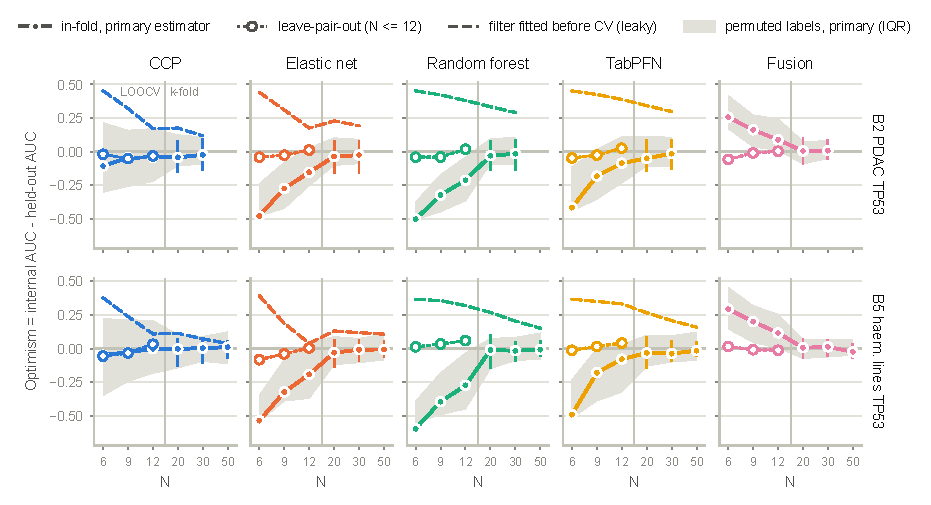
\includegraphics[width=\textwidth]{fig2_optimism.pdf}
\caption{Optimism (internal minus held-out AUC) by model and $N$, true labels. Solid: in-fold primary
estimator (pooled LOOCV for $N \le 12$, repeated 5-fold for $N \ge 20$; the vertical line marks the switch),
with its interquartile range as bars at $N \ge 20$. Dotted, open markers: leave-pair-out (post hoc for the
fusion network). Dashed: supervised filter fitted on all of $S_r$ before CV. Grey band: interquartile range
of the primary estimator under permuted labels. Medians over 100 repeats. B1 is omitted: every true-label
median is 0.00.}
\label{fig:optimism}
\end{figure}

\subsection{From $N = 20$, $k$-fold is right on average but often wrong in one study}
Per-fold $k$-fold meets the condition, and its median optimism for the four baselines lies between $-0.05$ and
$+0.01$. But the spread is wide (Figure~\ref{fig:optimism}, bars): internal AUC exceeds held-out AUC by more
than 0.1 in 13--26\% of repeats for single configurations, and in 17--23\% of all baseline repeats at
$N = 20$--$30$ (15\% at $N = 50$, B5). Little of that spread is noise in the held-out AUC itself: its
Hanley--McNeil variance \citep{hanley1982auc} accounts for only 7--21\% of the variance of optimism, so most of
it is error in the internal estimate. The pre-specified usable-$N$, the smallest $N$ from which median optimism
stays below 0.05, is not identifiable: it is $N = 6$ for 12 of 15 configurations in B2 and B5 only because
pooled LOOCV is pessimistic there, and a two-sided version lands mostly where the estimator switches ($N = 20$;
30 for four configurations in B2, earlier for CCP).

\subsection{Leaky pipelines inflate the estimate, and keep doing so}
Fitting the supervised filter on all of $S_r$ before CV raised the internal AUC of the four baselines well
above the held-out AUC (Figure~\ref{fig:optimism}, dashed): median optimism $+0.37$ to $+0.45$ at $N = 6$ and
still $+0.04$ to $+0.30$ at the largest $N$. The leaky SMOTE arms fit all preprocessing, that filter included,
and SMOTE on all of $S_r$, so they carry both leaks: median optimism $+0.37$ to $+0.45$ at $N = 6$ and $+0.22$
to $+0.36$ at the largest $N$, with internal AUCs of 0.96--1.00 even under permuted labels. Comparing them on
the same draws with the leaky pass of the in-fold SMOTE arms, which refits only the filter, separates the two
(\emph{post hoc}). At $N = 6$ the filter leak alone puts the internal AUC at its ceiling, and SMOTE adds
nothing; from $N = 20$, where the estimator is calibrated, SMOTE (with imputation and scaling also fitted on
all of $S_r$) adds a further $0.07$--$0.16$ (medians, positive in 95--100\% of draws), and $0.08$--$0.13$ at
the largest $N$. Each synthetic point interpolates between two real samples of one class, so
when SMOTE runs before the split, near-copies of every test sample, carrying its label, sit in its training
fold. SMOTE inside the training fold changed nothing: it never outranked its reference in any task.

\subsection{Model and pipeline rankings}
Figure~\ref{fig:ranking} shows mean ranks by held-out AUC. In both B2 and B5, the fusion network is outranked by
TabPFN from $N = 9$, by CCP and RF from $N = 12$, and by EN from $N = 20$, by a median of 0.04 to 0.19 AUC---secondary
claims. At $N = 6$ no pair meets the rule in both tasks (in B5 alone all four baselines outrank the fusion
network). Among CCP, EN, RF and TabPFN no pair meets the rule in both tasks; TabPFN outranks EN at every $N$ in
B5 but not in B2, a single-task result. The mean-rank orderings of B2 and B5 agree from $N = 9$, with or without
the fusion network (Kendall's $W$ 0.82--1.00), but the margins among the four baselines are too small for the
decision rule. Reactome pathway aggregation was outranked by protein features for RF at
$N = 9$, 12, 20 and 30 and for EN only at $N = 30$ (secondary claims); the variance filter, complete-case
proteins and in-fold SMOTE never outranked the reference pipeline in any task. Median held-out AUC rose from
0.55--0.56 at $N = 6$ to 0.63--0.65 at $N = 30$ in B2, and from 0.59--0.63 to 0.72--0.78 at $N = 50$ in B5, for
the four baselines (Supplementary Figure S1); the fusion network stayed at 0.49--0.59.

\begin{figure}[t]
\centering
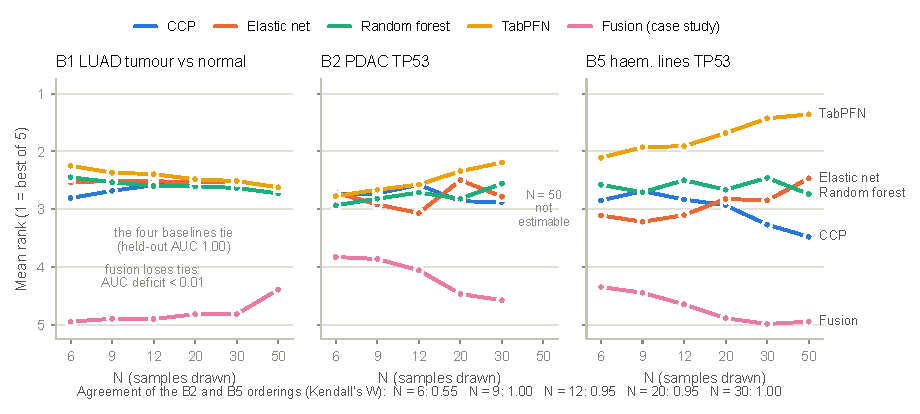
\includegraphics[width=\textwidth]{fig1_ranking.pdf}
\caption{Mean rank of the five models by held-out AUC within each repeat (1 = best; ties averaged), true
labels. In B1 every model is at ceiling and the fusion network loses ties by less than 0.01 AUC; no claim can
rest on B1.}
\label{fig:ranking}
\end{figure}

\subsection{Protein lists are barely reproducible, and stability does not predict recovery}
In B2 and B5, recovery of the full-cohort top 50 was small (Figure~\ref{fig:recovery}): precision@50 of
0.003--0.076 up to $N = 30$, against 0.002--0.014 under permuted labels. CCP reached 0.13 in B5 at $N = 50$; in
B1 it reached 0.19 at $N = 6$ and 0.66 at $N = 50$ (0.14 to 0.51 against the Wilcoxon reference), while EN, RF
and the fusion network stayed at 0.07--0.26. Recovered proteins almost always changed in the full-cohort
direction (0.90--1.00). $S_r$ makes up as much as 31\% of the reference data; against a reference computed on
$H_r$ alone (\emph{post hoc}), precision@50 at the largest $N$ fell (CCP: 0.056 to 0.029 in B2, 0.127 to 0.092
in B5). With that, and no FDR-significant protein in B2's reference, recovery is descriptive only.

Selection was close to irreproducible. For the supervised configurations in B2 and B5 up to $N = 30$, the
Kuncheva index of the top 50 between different subsamples was 0.00--0.04 (0 = chance overlap), likely an overestimate. In B1 it was 0.02--0.18 for EN and RF, despite perfect classification, while CCP rose
from 0.11 to 0.56. The variance-filter arms were at least as stable under permuted labels (0.02--0.09) as the
supervised arms of B2 and B5 under true labels, because their selection ignores the labels: stability can be
high with no signal at all. The pre-specified test of whether stability predicts recovery passed:
Spearman $\rho$ across (configuration, $N$) cells with $N \le 30$ was 0.58, 0.58 and 0.71 in B1, B2
and B5, all above the 0.5 bar. But $N$ alone correlates with recovery at 0.52, 0.91 and 0.89, and once
stability and recovery are ranked within each $N$---the situation of a laboratory at one $N$---$\rho$ falls to
0.39, 0.10 and 0.41, with single-$N$ values as low as $-0.65$ (Supplementary Figure S2). We do not claim that
stability is a usable proxy for recovery.

\begin{figure}[t]
\centering
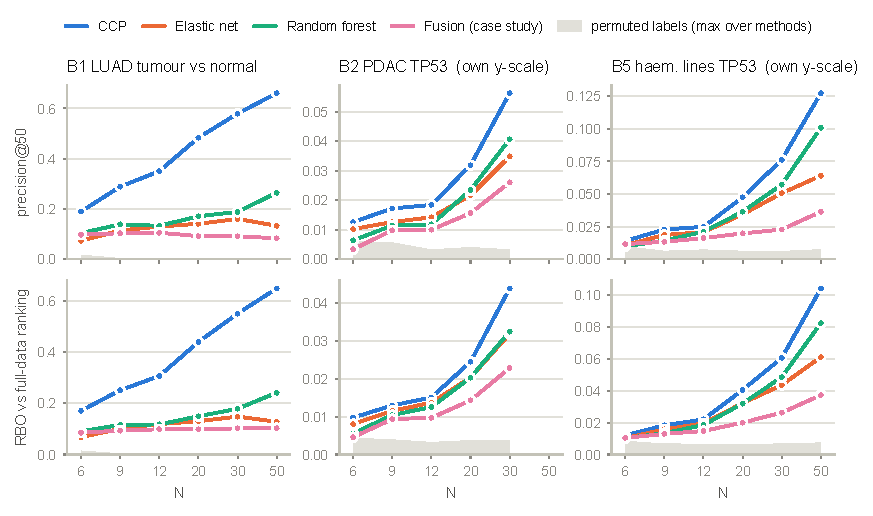
\includegraphics[width=\textwidth]{fig4_recovery.pdf}
\caption{Biomarker recovery against the full-cohort limma ranking, true labels, mean over 100 repeats. Grey:
largest value under permuted labels. B2 and B5 use their own $y$-scales. TabPFN and pathway arms have no
protein ranking.}
\label{fig:recovery}
\end{figure}

\subsection{Follow-up runs: embeddings add nothing, outside labels help}\label{sec:posthoc}
After the benchmark, five follow-up runs, each fixed in a written plan before fresh draws (repeats 100--599;
Supplementary Table~S2), asked what raises held-out AUC at $N = 12$ and 30. A denoising variant of the fusion network with
multiplicative fusion did no better with ESM-2 embeddings, their 32- or 64-dimensional
principal components, or co-expression components from 786--859 independent samples than with the same
embeddings shuffled across proteins (median differences $-0.021$ to $+0.009$); letting inner CV set an
embedding's weight in a ridge model changed held-out AUC by a median of 0.000. Outside label information did
help. A TP53 signature fitted to other CPTAC cohorts (B2) or other ProCan tissues (B5), applied without the
study's labels, reached a median held-out AUC of 0.70 (B2) and 0.77 (B5) at $N = 12$ and beat all four
baselines at $N = 12$ and 30 in both tasks (by 0.04--0.11 over TabPFN); TabPFN caught up only at $N = 50$ in
B5. Used as a prior for ridge on the 500 proteins the study's filter kept, it beat plain ridge only in B5 at
$N \ge 30$.

% =====================================================================================
\section{Discussion}\label{sec:discussion}

\begin{table}[!t]
\centering
\caption{Decision table for small proteomic studies, from the two weak-signal tasks (B2, B5) except the last
row (B1). Evidence: \emph{secondary claim} = paired decision rule holds in both B2 and B5, a post hoc
relaxation of the pre-specified rule (\S\ref{sec:results}); \emph{descriptive} = measured and consistent in
both, with no pre-specified decision rule; \emph{follow-up test} = hypothesis fixed before fresh draws after the
benchmark (\S\ref{sec:posthoc}); \emph{none} = no basis to choose. A small study cannot tell a weak
effect from none with its own data (\S\ref{sec:tasks}); unless its effect is known to be large, it should
follow the rows as they stand.}
\label{tab:decision}
\begin{tabularx}{\textwidth}{@{}l l X l@{}}
\toprule
$N$ & Question & Recommendation & Evidence \\
\midrule
$\le 12$ & Internal estimate & Report leave-pair-out AUC, not pooled LOOCV (errors $-0.60$ to $+0.29$ vs.\ $\pm 0.08$) & descriptive \\
$\ge 20$ & Internal estimate & Repeated $k$-fold, AUC per fold; expect $>0.1$ overstatement in about one study in five (17--23\% at $N = 20$--30) & descriptive \\
all & Own null & Re-run the whole pipeline on permuted labels with leave-pair-out or per-fold $k$-fold; a mean well above 0.5 exposes a leak (at 3 vs 3 only 20 labellings exist, so a permutation $p$ cannot fall below 0.05, or 0.1 for label-symmetric pipelines) & descriptive \\
all & Feature selection & Inside the folds only (outside: $+0.04$ to $+0.45$ optimism) & descriptive \\
all & Augmentation & Never before the split (SMOTE adds $0.07$--$0.16$ from $N = 20$ on top of other leaks); inside the folds it does not help & descriptive \\
9--30 & Model & Avoid the fusion network (TabPFN better from $N = 9$, CCP and RF from 12, EN from 20; by 0.04--0.19 AUC) & secondary claim \\
6--30 & Model & No basis to choose among CCP, elastic net, random forest, TabPFN & none \\
$\le 30$ & Outside information & If a labelled cohort exists for the same contrast, score with its signature: it beat all four standard models at $N = 12$ and 30; protein embeddings added nothing & follow-up test \\
9--30 & Features & With RF, use proteins, not pathway scores (EN: $N = 30$ only) & secondary claim \\
$\le 30$ & Biomarker list & Do not read the top 50 as a biomarker list (Kuncheva 0.00--0.04) & descriptive \\
$\le 30$ & Stability & Not a proxy for recovery at a fixed $N$, and high even with no signal & none \\
any & Large effect & Every method reaches a median AUC of 0.99--1.00 from $N = 6$ (B1, full-cohort $|d| \approx 4$); no basis to choose & none \\
\bottomrule
\end{tabularx}
\end{table}

Table~\ref{tab:decision} turns the results into recommendations. The most robust finding concerns the
estimator, as Proposition~\ref{prop:null} predicts. A laboratory reporting pooled leave-one-out AUC at $N \le 12$ reports a number whose
error depends on the classifier more than on the data, and whose sign it cannot know without a permuted-label
run. Leave-pair-out costs more fits but removes almost all of the error. From $N = 20$, $k$-fold is centred
correctly, but about one study in five still overstates its held-out AUC by more than 0.1. The two leaky practices we measured are not small-$N$ curiosities: both still inflate the estimate
at $N = 30$--50. No model was reliably best among the four baselines, no pipeline variant helped, and the
case-study fusion network was the weakest model wherever methods could be separated. A small study whose contrast has been measured in a labelled public cohort should first score its samples with that cohort's signature (\S\ref{sec:posthoc}): its labels play no part in that fit, so the AUC is a genuine held-out estimate. At $N \le 30$, different
subsamples selected nearly disjoint protein lists, so a small study's top-ranked proteins are hypotheses from
one draw, not a panel.

\subsection{An illustration on the motivating study}\label{sec:case}
The nine-sample study cannot measure optimism, but it shows how the two internal estimators behave at the
bottom of the range. Each of its three binary contrasts has three samples per class ($N = 6$).
For each, we analysed all ten distinct 3/3 partitions of the six samples, the true one and nine rearrangements, with the
benchmark's reference pipeline and five models (Figure~\ref{fig:case}); no claim rests on it.

Three things stand out. First, the true 24-hour versus control partition reaches an internal AUC of 1.00 for
every model under both estimators. Missingness rises with exposure (24.2\%, 60.6\% and 78.1\% of values), and
the per-sample missing fraction alone, with no model, separates all three contrasts perfectly (\emph{post hoc};
24 versus 8 hours by only 0.1 percentage point), so a perfect internal score need not reflect protein-level
signal. Second, on the same data and model the two estimators can disagree
sharply: for 24 hours versus 8 hours, leave-pair-out gives 1.00 for every model, while pooled LOOCV gives 0.33
to 1.00, the fusion network's own value being 0.33. Third, across the 27 rearranged partitions, pooled LOOCV
values pile up near zero (median 0.22 over 135 values, 46\% at or below 0.2), while leave-pair-out stays nearer
the middle (median 0.44, 12\%), as the benchmark measured. One six-sample dataset need not reproduce each
method's benchmark direction, so we read the figure only as showing that the choice of estimator alone can
move a small study's headline number by more than half the AUC scale. For that study, internal estimates alone cannot
establish generalisation, and its top-ranked proteins are hypotheses from one draw.

\begin{figure}[t]
\centering
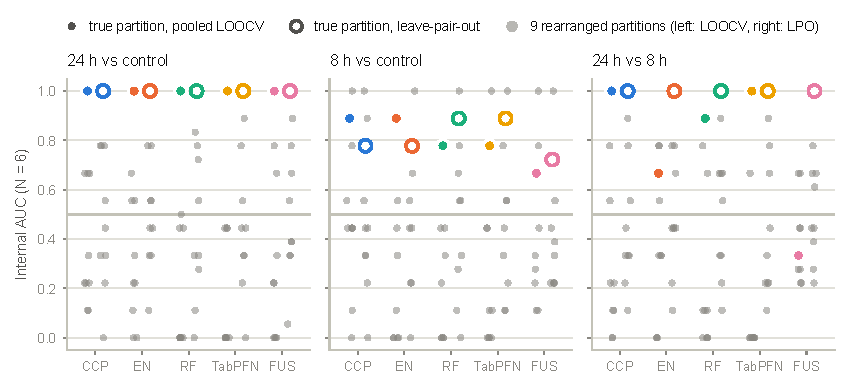
\includegraphics[width=\textwidth]{fig6_case_study.pdf}
\caption{Internal AUC on the motivating study for the three binary contrasts ($N = 6$). Coloured markers: the
true partition, by pooled LOOCV (filled) and leave-pair-out (open). Grey: the nine rearranged 3/3 partitions
(left of each pair: pooled LOOCV; right: leave-pair-out). Descriptive; added after the benchmark results were
known.}
\label{fig:case}
\end{figure}

\subsection{Limitations}
The conclusions transport only as far as the tasks. Only B2 and B5 discriminate between methods; both are weak
TP53 contrasts in cancer material, chosen by a rule (smallest effect) whose statistic could not order them
(\S\ref{sec:tasks}). None is plasma, the most common small-$N$ setting, or label-free DDA, the motivating study's platform (B1 and B2 are TMT, B5 is DIA). Missingness in the benchmark barely depends on the label (the per-sample
missing fraction separates the classes with AUC 0.46--0.65), unlike in the motivating study, so pipelines under strongly label-dependent missingness are untested. $H_r$ comes from
the same cohort as $S_r$; optimism against a truly independent cohort, with other sites and batches, is likely
larger. All draws were balanced and all models ran at default settings, so class imbalance and nested tuning
were not studied, nor were bootstrap estimators such as .632+ \citep{efron1997improvements} or Harrell's
optimism correction \citep{harrell1996multivariable}. The fusion network ran on the reference pipeline's
500-protein input, not the original study's full protein set, and the motivating study was three-class
whereas every task is binary. The transferred signature needs labelled data for the same contrast, which TP53
has and the motivating study's exposure does not, and in both tasks the outside cohorts shared the task's
platform and processing, so transfer across platforms is untested.

\FloatBarrier
\section{Conclusion}
A symmetry condition guarantees calibrated internal AUC under uninformative labels and explains why pooled
leave-one-out AUC errs in a direction set by the learner. At
wet-lab sample sizes, the estimator and the pipeline move the reported AUC far more than the choice among
standard models, and at $N = 12$ and 30 a signature from outside labelled data scored higher than the four
standard models trained on the study. We recommend leave-pair-out
AUC at $N \le 12$, a permuted-label run of the full pipeline, strictly in-fold selection and augmentation, a
signature from a labelled external cohort where one exists, and caution in reading short protein lists as
biomarker panels.

\paragraph{Data and code availability.} All three cohorts are public (CPTAC via the \texttt{cptac} package
\citep{lindgren2021cptac}; ProCan-DepMapSanger via figshare \citep{goncalves2022procan}). The code,
leakage tests, analysis scripts, complete results and the follow-up runs with their plans (\texttt{posthoc/})
are at \coderepo.
The motivating nine-sample dataset (\S\ref{sec:case}),
generated by the collaborating laboratory, is available from the authors on reasonable request.

\bibliographystyle{unsrtnat}
\bibliography{refs}

\end{document}
